%%%%%%%%%%%%%%%%%%%%%%%%%%%%%%%%%%%%%%%%%%%%%%%%%%%%%%%%%%%%%%%%%%%
%
% Dissertationen mit LaTeX auf dem edoc-Server
%
% Humboldt-Universitaet zu Berlin
% Computer- und Medienservice
% Arbeitsgruppe Elektronisches Publizieren
% Bezug der Vorlage und der Richtlinien:
%     http://edoc.hu-berlin.de/e_autoren/latex/
%
% Kontakt:
%     E-Mail:
%                   edoc-latex@rz.hu-berlin.de
%     Telefon:              siehe
%     http://edoc.hu-berlin.de/e_autoren/latex/kontakt.php  %
%
%%%%%%%%%%%%%%%%%%%%%%%%%%%%%%%%%%%%%%%%%%%%%%%%%%%%%%%%%%%%%%%%%%%%%%%
%
% Das folgende Template muss f�r die Publikation von digitalen        %
% Dissertationen in LaTeX an der Humboldt-Universit�t benutzt werden. %
%
% Aendern Sie den Name dieser Datei auf ihren_nachname.tex.           %
%
% Die mit einem Stern (*) gekennzeichnete Teile sind optional;        %
% falls Sie sie nicht verwenden m�chten, sind entsprechende Zeile       %
% zu entfernen.
%
%%%%%%%%%%%%%%%%%%%%%%%%%%%%%%%%%%%%%%%%%%%%%%%%%%%%%%%%%%%%%%%%%%%%%%%

% \listfiles    % Erstellt eine Liste von allen benutzten Dateien
% zusammen mit ihrer Versionen
% und ggf. einer kurzen Beschreibung
% Sie wird in die log-Datei geschrieben

\documentclass[12pt,a4paper% die Verwendung von DIN-A4-Format ist pflicht!
]{report}
\usepackage[top=2cm, bottom=2.5cm, left=3cm, right=3cm]{geometry}

%notwendige Pakete
\usepackage[ngerman, english]{babel}    % mehrsprachiger Textsatz
% babel: letzte Sprache in Optionen zeigt die Sprache des Dokumentes
% und kann durch den Befehl \selectlanguage{} geaendert werden
% Passen Sie die Optionen des babel-Paketes nach Bedarf an!
\usepackage[latin1]{inputenc}       % Eingabekodierung Parameter latin1 darf ge�ndert werden
\usepackage[T1]{fontenc}                % Schriftenkodierung
\usepackage{graphicx}                       % zum Einbinden von Grafiken
\usepackage{lmodern}                        % Ersatz fuer Computer Modern-Schriften                                        zum besseren Aussehen am Bildschirm
\usepackage{cite}
\usepackage{amssymb}
\usepackage{amsmath}
%\usepackage{float} %to keep tables where they should be	
%\usepackage{bm}
\usepackage[bottom]{footmisc} %to keep footnotes at the bottom (not glued under the text)
\usepackage{todonotes}

%-Eingabe der Metadaten des Titelblattes--------------------------

%-Daten des Autors / Authors Data---------------------------------

\newcommand{\dcauthorpre}{~} 
\newcommand{\dcauthorsurname}{Bothe} 
\newcommand{\dcauthorname}{Marius} 
\newcommand{\dcauthoradd}{born 23. February 1995}

%-Titel und Untertitel / Title and subtitle-----------------------

\newcommand{\dctitle}{Asymptotic Behavior of L\'evy Walks} 
\newcommand{\dcsubtitle}{~}  
% Falls dcsubtitle NICHT verwendet werden soll, {\dcsubtitle}{~} eingeben.

%-Eingabe der Betreuuernahmen / Names of the consultants---------

\newcommand{\dcconsulta}{Prof. Dr. Igor Sokolov} 
\newcommand{\dcconsultb}{~} 
\newcommand{\dcconsultc}{~} 

%-Eingabe der Gutachternamen / Names of the approvals-------------

\newcommand{\dcapprovala}{Prof. Dr. Igor Sokolov} 
\newcommand{\dcapprovalb}{Dr. Michael Zaks} 
\newcommand{\dcapprovalc}{~} 

%-Information zur Universitaet------------------------------------

\newcommand{\dcdegree}{Master of Science\\(M. Sc.)} 
\newcommand{\dcsubject}{Physics} 
\newcommand{\dcfaculty}{Mathematisch-Naturwissenschaftliche Fakult\"at I}
\newcommand{\dcinstitute}{Institut f\"ur Physik}
\newcommand{\dcuniversity}{Humboldt-Universit\"at zu Berlin}
\newcommand{\dcdean}{Prof. Dr. Elmar Kulke}
\newcommand{\dcpresident}{Prof. Dr.-Ing. Dr. Sabine Kunst }

%-Pruefungsdaten: eingereicht und mdl. Pruefung-------------------
%-data of submission and oral exam--------------------------------

\newcommand{\dcdatesubmitted}{XXXXXXXXXX} %auch wenn nicht auf dem Titelblatt, bitte erf�llen!
\newcommand{\dcdateexam}{???} 

%-deutsche Schlagwoerter / german keywords------------------------

\newcommand{\dckeydea}{~}
\newcommand{\dckeydeb}{~}
\newcommand{\dckeydec}{~}
\newcommand{\dckeyded}{Schlagwort}

% Folgende Zeile bitte nicht aendern!
\newcommand{\dckeywordsde}{\vfill \raggedright {\textbf{Schlagw\"orter:}}\\ \dckeydea, \dckeydeb, \dckeydec, \dckeyded \\}

%-englische Schlagwoerter / english keywords----------------------

\newcommand{\dckeyena}{keyword 1}
\newcommand{\dckeyenb}{~}
\newcommand{\dckeyenc}{~}
\newcommand{\dckeyend}{~}

% Folgende Zeile bitte nicht aendern!
\newcommand{\dckeywordsen}{\vfill \raggedright {\textbf{Keywords:}}\\ \dckeyena, \dckeyenb, \dckeyenc, \dckeyend \\}

\newcommand{\dcpdfsubject}{Dissertation}                          % Bitte ALLE Angaben erf�llen!
\include{compatibility}

\usepackage{glossaries}


%-Eigene Trennregeln*---------------------------------------------

% \include{hyphenations}

% Custom Commands-----------------------------------------

\makeatletter
\def\@makechapterhead#1{% Damit "Chapter 1" etc. nicht mehr angezeigt wird
  \vspace*{50\p@}%
  {\parindent \z@ \raggedright \normalfont
    \interlinepenalty\@M
    \Huge\bfseries  \thechapter.\quad #1\par\nobreak
    \vskip 40\p@
  }}
\makeatother

\newcommand{\ve}[1]{\mathbf{ #1 }}

\newcommand{\abs}[1]{\ensuremath{\left|\,#1\,\right|}}
%                                          % absolute value, |...|
%
\newcommand{\diff}[1]{\ensuremath{\textrm{d}#1}}
%                          % as \rmd, but expecting as argument the
%                          % corresponding variable, like df
%
\newcommand{\der}[2]{\ensuremath{\dfrac{\text{d}#1}{\text{d}#2}}}
%                      % derivative like df / dx
%
\newcommand{\nder}[3]{\ensuremath{\dfrac{\text{d}^{#3}#1}{\text{d}#2^{#3}}}}
%                      % nth derivative like d^n f / dx^n
%
\newcommand{\pder}[2]{\ensuremath{\dfrac{\partial#1}{\partial#2}}}
%                      % partial derivative like \partial f / \partial x
%
\newcommand{\npder}[3]{\ensuremath{\dfrac{\partial^{#3}#1}{\partial#2^{#3}}}}
%                      % nth partial derivative, \partial^n f / \partial x^n
%

%Glossary, uses custom commands
\setacronymstyle{long-short}
%Acronyms
\newacronym{msd}{MSD}{mean squared displacement}
\newacronym{ctrw}{CTRW}{continuous time random walk}

%Glossaryentries
\newglossaryentry{x2}{name={\langle x^2 \rangle},description={means squared displacement}}

%-Dokument--------------------------------------------------------

\begin{document}

% Es muss zitiert werden k�nnen! Im Vorspann roemisch,
% Im Hauptteil benutzt man arabische Nummerierung.
\pagenumbering{roman}

%-Titelblatt------------------------------------------------------

%----------Generierung der Titelseite-----bitte nicht ver�ndern!--------------------


\author{by \\ \dcauthorpre\ \dcauthorname\ \dcauthorsurname\ \\ \dcauthoradd}

%----------
\title{ \vspace{-4cm}\dctitle \\ 
\vspace{0.5cm}
\large{\dcsubtitle} \\ 
\vspace{0.5cm} {\Large{BACHELOR THESIS}}\\ 
\vspace{0.5cm} \large{for attaining the academic grade of \\ 
\dcdegree\\ in the field of \dcsubject \\\vspace{0.5cm}
\includegraphics[width=6cm]{husiegel}\\ 
\vspace{0.5cm} submitted to \\ 
\dcfaculty \\ 
\dcinstitute\\
\dcuniversity \\}}
%-----------------
\date{\vspace{2.5cm}
%\raggedright{
%Pr\"asident der Humboldt-Universit\"at zu Berlin:\\
%\dcpresident \vspace{-0.3cm}
%}\vspace{0.5cm}\\
%
%\raggedright{
%Dekan der \dcfaculty:\\
%\dcdean \vspace{-0.3cm}
%}\vspace{0.5cm}\\
%
% auskommentiert weil nicht standard
%\raggedright{
%Gutachter:
%\begin{enumerate} 
%\item{\it\dcapprovala} \vspace{-0.3cm}
%\item{\it\dcapprovalb} \vspace{-0.3cm}
%\item{\it\dcapprovalc} \vspace{-0.3cm}
%\end{enumerate}} \vspace{0.5cm}
\raggedright{
Supervising tutors:
\begin{enumerate} 
\item{\it\dcapprovala} \vspace{-0.2cm}
\item{\it\dcapprovalb} \vspace{-0.2cm}
\end{enumerate}} \vspace{0.3cm}
%-----------------
\raggedright{
\begin{tabular}{lll}
Submitted on: &  &\it\dcdatesubmitted\\ % wenn nicht in der Pr�fungsordnung, die Zeile bitte auskommentieren
%Tag der m\"undlichen Pr\"ufung: & & \dcdateexam
\end{tabular}}\\ 
}
%-------------------------------------                         % Bitte KEINE �nderungen vornehmen!
\maketitle


%-Zusammenfassung / Abstract*-------------------------------------

%%-englische-Zusammenfassung---------------------------------------

\selectlanguage{english}

\begin{abstract}
\setcounter{page}{2} % Nach Bedarf anpassen!

The topic of this thesis is the connection between Yang-Mills and Einstein-Yang-Mills amplitudes.\\
Recently a number of different relations between the two have been found in the CHY representation by de la Cruz, Kniss and Weinzerl\cite{weinzerl16} as well as by Nandan, Plefka, Schlotterer and Wen \cite{plefka16}. \\
In the following a brief derivation of the formula presented in \cite{weinzerl16} and \cite{plefka16} is given and the equivalence of the two approaches in the 4 and 5-point cases with 1 and 2 gravitons is shown explicitly.




% hier werden die englische Schlagw�rter aus Metadaten �bernommen
\dckeywordsen				
\end{abstract}




\selectlanguage{english}               % Bitte an die Sprache denken!!!
\setcounter{page}{2}                   %   Bitte an die Seitenzahl denken!!!

%-Widmung*--------------------------------------------------------

%\include{dedication}

%-Inhaltsverzeichnis----------------------------------------------

\tableofcontents
\pagebreak

%\listoffigures
%\pagebreak

%\listoftables

%-Hauptteil-------------------------------------------------------

\pagenumbering{arabic}
\pagestyle{plain}                  % bzw. ist fancyhdr zu benutzten

%-Kapitel---------------------------------------------------------

% part ist optional, bitte ggf. l�schen
% \part{Teil1}

\include{chapter01} %Introduction
\chapter{Theoretical Background}

\section{The model}

\subsection{L\'evy walks}

The original motivation for the creation of the L\'evy walk model goes back to the work of Richardson in 1926 \cite{richardson}, who studied the motion of particles in the turbulent flow of the atmosphere. Such a system contains jets and eddies that affect the behavior of the particle and lead to anomalous diffusion. In particular Richardson found that the \gls{msd} of the particle scales with the third power of the time, i.e.

\begin{align}
\gls{x2}(t) \propto t^3 ,
\end{align}
%
which is known as the Richardson regime.\\

There were several attempts to find a random walk model that replicates this behavior. These attempts found that power-law models were particularly suitable for describing superdiffusion \footnote{meaning diffusion where $\gls{x2}(t) \propto t^{1+\alpha}$, $\alpha>0$} which lead to the creation of the L\'evy flight model: In this model the walker jumps instantaneously in a random direction with a jump length drawn from a distribution $g(\abs{\ve{x}})$. He now waits at the turning point for the duration of the waiting time, which is drawn from the distribution $\gls{psi}(t)$ and then performs a new jump in another direction, as can be seen in figure (\ref{fig:levyFlight}). Both the waiting time and the jump length distributions are power-laws, meaning for large arguments they take the form 

\begin{align}
\gls{psi}(t) \propto t^{-1-\gamma}, \qquad g(\abs{\ve{x}}) \propto \abs{\ve{x}}^{-1-\beta}, \qquad \gamma, \beta > 0.
\end{align} 
%
\begin{figure}
\begin{center}
\includegraphics[width=90mm]{pics/levyFlight.png}
\caption{Comparison between the trajectories of the one dimensional L\'evy flight and L\'evy walk (for $\nu=1$). Note that the jump length of the L\'evy flight is independent of the waiting time. 
\label{fig:levyFlight}}
\end{center}
\end{figure}
%
However the L\'evy flight model has a major drawback: Since the jumps happen instantaneously it has an infinite propagation speed, which causes its \gls{msd} and all higher moments to diverge \cite{lwreview}. \\


Therefore the L\'evy walk model was developed by Shlesinger, Klafter and West \cite{shlesinger1987}. Here the walker no longer waits at the turning points, but his jumps now have a finite duration, turning them into steps. The step duration is coupled to the length of the step and prevents the infinite propagation speed that caused problems with the L\'evy flights, which is illustrated in figure \ref{fig:levyFlight}. \\

The path of a walker in the new model is now described by a series of step durations $\gls{dur}_1, \gls{dur}_2, ...$ which are drawn from the power-law distribution 

\begin{align}
\gls{psi}(\gls{dur}_i) = \frac{\gamma}{t_0} \frac{1}{(1+\gls{dur}_i/t_0)^{\gamma+1}} .
\end{align}
%
Here the parameter $\gamma>0$ governs the width of the distribution and { \color{red}$t_0$ is the timescale of a step }. These step durations are associated with their respective steps vectors $\ve{x}_1, \ve{x}_2, ...$, whose direction is chosen randomly. By partially summing up the step durations and the step lengths one obtains the turning times $\gls{ttime}_n$ and the turning points $\gls{tpoint}_n$ respectively:

\begin{align}
\gls{ttime}_n = \sum_{j=1}^n \gls{dur}_j , \qquad \gls{tpoint} = \sum_{j=1}^n \ve{x}_j
\end{align}
%
The walker is now being observed at the observation time $t$: Let the last turning time before $t$ be $\gls{ttime}_n = \text{ max} \{\gls{ttime}_i | \gls{ttime}_i \leq t \}$, then the distance covered from the last turning point is given by

\begin{align}
\abs{\ve{x}_{n+1}} = c (\gls{dur}_{n+1})^{\nu-1} (t-\gls{ttime}_n) ,
\end{align}
%
where c is a constant with dimension $ [ s t^{-\nu} ] $ . The speed 

\begin{align}
\gls{speed} = \pder{}{t} \abs{\ve{x}_{n+1}} = c (\gls{dur}_{n+1})^{\nu-1}
\end{align}
%
is therefore constant during the entire step but depends on the step duration $\gls{dur}_{n+1}$, where the parameter $\nu>0$ governs this dependence. \\
For any completed step we can now write down the joint probability to make a step of length $\abs{\ve{x}}$ and duration $\gls{dur}$:

\begin{align}
\gls{psi}(\ve{x}, \gls{dur} ) = \frac{\gamma}{t_0} \frac{1}{(1+\gls{dur}/t_0)^{\gamma+1}}  \frac{\delta(\abs{\ve{x}} - c \gls{dur}^{\nu}) }{\abs{\gls{step}}^{d-1} \abs{S^{d-1}}}  .
\end{align}
%
Here $d$ is the spatial dimension of the process and $\abs{S^{d-1}}$ is the surface area of a d-dimensional unit ball. Note that both the step duration distribution and the joint distribution are denoted by $\gls{psi}$, but their arguments are different. In conclusion we have a model that is governed by two parameters, $\nu$ and $\gamma$ and can produce different kinds of anomalous diffusion.\\

Because of this versatility the L\'evy walk model is used to describe a variety of systems: Besides the application in turbulent systems for which the model was originally invented it finds application in field like biology, where  the special case of fixed velocities ($\nu=1$) is used to approximate the motion of E. coli bacteria, who move with the help of microscopic flagella. These flagella either rotate in a synchronized manner, which leads to long stretches of relatively fast movement, or unsynchronized, which leads to a tumbling motion in which the bacterium changes its direction. The resulting motion was found to follow a power-law distribution with parameter $\gamma = 1.2$ \cite{korobkova2004}

\todo{more examples: light scattering, chaotic Hamiltonian systems}



However it was found recently in \cite{radons2018} that the \gls{msd} of the model is actually divergent for certain values of its parameters, a fact that had previously gone unnoticed for the three decades of the models existence. 
The divergence can be seen directly when one writes down the contribution to the second moment of the distribution from the trajectories, that consist only of a single step longer than the observation, i.e. where the particle never stops:

\begin{align}
\gls{x2}(t) \geq& \int_{\mathbb{R}^d} \int_{t}^{\infty} \abs{\gls{step}}^{2}(t') \gls{psi}(\gls{step},t') dt' d^{d}x \\
=& \frac{\gamma}{t_0} \int_{0}^{\infty} \int_{t}^{\infty} \abs{\gls{step}}^{2}(t')  \frac{1}{(1+t'/t_0)^{\gamma+1}}  \delta(\abs{\gls{step}} - c (t')^{\nu-1}t)  dt' d\abs{\gls{step}} \\
=& \frac{\gamma t^2}{t_0}  \int_{t}^{\infty}   \frac{c^2 (t')^{2\nu-2}}{(1+t'/t_0)^{\gamma+1}}    dt'  .
\end{align}
%
The integrand is proportional to $(t')^{2\nu-\gamma-3}$, therefore the integral will diverge at infinity whenever $2 \nu \geq \gamma +2$ holds. This includes the parameter region where the Richardson regime was expected, so the model that was essentially invented to cure the divergence in the description of the Richardson regime turns out to be divergent itself. In order to remedy this, a more general model model is necessary, whose investigation will be the focus of this thesis.
% problem: divergence from radons

\subsection{Generalized L\'evy walks}

%mention drude model of Sokolov
% interpolation via eta
% formulate model 
% picture
% general properties

% Further generalizations of the model

\section{Theory of random walks}

\subsection{Continuous time random walks}

%zoom in from RW -> CTRW -> space-time coupled CTRWs

% introduce laplace tf

% introduce: survival probability, forward waiting time, step rate, mean number of steps 

% derive formula for number of steps 

% derive formula for total pdf

\subsection{Space-time coupled continuous time random walks}

 %Theoretical Background
\chapter{Theoretical Background and Methodology} %Methodology
\include{chapter03} %Analytical Calculations
\chapter{Results and Discussion}

%MSD: analise regions of behavior along the lines of where step length and step variance diverge %Results and Discussion
\chapter{Conclusions}

 \cite{plefka16} %Conclusions
% usw.

%-Anhang----------------------------------------------------------

\appendix

%-Literaturverzeichnis--------------------------------------------

%\nocite{*}
%die Verwendung von bibtex ist Pflicht!!!
\bibliography{bibliography}
\bibliographystyle{unsrtdin}        %bzw. unsrtdin, alphadin, abbrvdin

%-Kapitel des Anhangs---------------------------------------------

%\chapter{The Tauberian theorem} \label{sec:tauberian}

In this thesis we frequently consider Laplace transforms of functions asymptotically following power laws. The asymptotic form of Laplace transforms of functions which at long times behave as $f(t) = t^{\rho-1} L(t)$, where $L(t)$ is a slowly varying function, in the asymptotic regime $s \to 0$ as well as the corresponding inverse transforms may be obtained by use of the Tauberian theorem. Note that the following derivation is taken from \cite{bothe}.\\

We assume that a Laplace transform $f(s) = \int_0^t f(t) e^{-st} dt$ exists, i.e. the function $f(t)$ does not possess a strong divergence at 0. All functions $f(t)$ appearing this thesis are non-negative. For such functions Laplace transforms are monotonically decaying functions of $s$. Depending on the behavior of $f(t)$ at infinity two cases should be considered: \\
The function $f(t)$ might be integrable on $[0, \infty)$, so that 
$\int_0^\infty f(t) dt = I_0^{f} < \infty$, or this integral may diverge. The first case corresponds to $\rho < 0$ and 
the second one to $\rho > 0$ (the case $\rho = 0$ may belong to the either class depending on the concrete form of $L(t)$). \\
In the second case the Tauberian theorem may be applied immediately, stating that if $f(t)$ is a regularly varying function, i.e. when  its Laplace transform is given by 
\begin{equation}
 f(t) \simeq t^{\rho-1} L(t) \;\; \leftrightarrow \;\; f(s) \simeq \Gamma(\rho) s^{-\rho} L\left(\frac{1}{s}\right)
 \label{eq:Tauberian}
\end{equation}
for $\rho \geq 0$. As in the main text, all slowly varying functions will be omitted (i.e. changed for constants $L$). 

We note that for $\rho < 0$  equation, i.e. when $f(t)$ is integrable, equation (\ref{eq:Tauberian}) suggests $f(s)$ being a growing function of $s$ and is therefore wrong. In this case let us consider the function
\begin{equation}
 S(t) = \int_t^\infty f(t') dt'.
\end{equation}
The integrability of $f(t)$ means that $S(t)$ is well-defined, and that $I_0^{f} =  \int_0^\infty f(t') dt' = S(0)$ is finite. 
The function $S(t)$ has the power-law asymptotics
%
\begin{equation}
 S(t) \simeq - \frac{L t^\rho}{\rho},
\end{equation}
and, if this is no more integrable (i.e. for $\rho > -1$), can be transformed via the Tauberian theorem, so that
\begin{equation}
 S(s) \simeq - L \frac{\Gamma(\rho+1)}{\rho} s^{-(\rho +1)} = - L \Gamma(\rho)  s^{-(\rho +1)},
\end{equation}
%
where in the last equality the identity $\Gamma(x+1) = x \Gamma(x)$ was used. 
Noting that $f(t) = - \frac{d}{dt}S(t)$ and using the Laplace representation of the derivative, we get 
\begin{equation}
 f(s) = S(t=0) - s S(s) = I^{f}_0 - L \Gamma(\rho)  s^{-\rho} .
\end{equation}
The direct application of the Tauberian theorem would give us a correct form of the second term (up to a sign), but omit the first one. 

If $S(t)$ is still integrable, we consider the function $P(t) = \int_t^\infty S(t') dt'$, whose power-law asymptotics for $t \to \infty$ is
\begin{equation}
 P(t) \simeq \frac{L t^{\rho+1}}{\rho (\rho+1)},
\end{equation}
and whose connection to $f(t)$ is given by $f(t) = \frac{d^2}{dt^2}S(t)$. For $-2 < \rho$ the function $P(t)$ is not integrable, 
and the application of the Tauberian theorem gives
\begin{equation}
 P(s) = L \frac{\Gamma(\rho+2)}{\rho (\rho+1)} s^{-\rho-2} = L \Gamma(\rho) s^{-\rho-2}.
\end{equation}
Using the Laplace representation for the second derivative we get
\begin{equation}
 f(s) = - s P(t=0) - P'(t=0) + s^2 P(s). 
\end{equation}
The value of $P'(t=0)$ is $-S(t=0)=-I^{f}_0$. The value $P(t=0)$ is given by the integral
\begin{equation}
P(t=0) = \int_0^\infty dt \int_t^\infty f(t')dt'.
\end{equation}
Changing the sequence of integrations in $t$ and $t'$ we get 
\begin{equation}
 P(t=0) = \int_0^\infty dt' f(t') \int_0^{t'} dt = \int_0^\infty t' f(t') dt'.
\end{equation}
Since $f(t)$ decays with $t$ faster than $t^{-2}$, the integral converges, and will be denoted by $I^{f}_1$. Therefore we have
%
\begin{equation}
 f(s) = I^{f}_0 - s I^{f}_1 + L \Gamma(\rho) s^{-\rho}.
\end{equation}

For $\rho < -2$ the procedure has to be repeated again for the function being the integral of $P(t)$, etc. The general result is
%
\begin{align}
 f(s) = \sum_{k=0}^{k_{\max}} \frac{(-1)^k}{k!} I^{f}_k s^k + L \Gamma(\rho) s^{-\rho}
\end{align}
%
with $k_{\max}$ being the whole part of $-\rho$, and $I^{f}_k$ being the moment integral
\begin{align}
I^{f}_k = \int_0^\infty t^k f(t) dt.
\end{align}
In the main text we never have to use more than first three terms of this expansion. 


\chapter{Estimates for the integral $I_{a,b,c}(y)$ \label{sec:integral}} 

We are interested in the integral 
%
\begin{eqnarray}
I_{a,b,c}(y) &=& \int^{1}_0 (1-z)^{b} [(z+y)^c-z^c]^2 (z+y)^{a}  dz \label{eqn:Iabc1} \\ 
&=& \int^{1}_0 (1-z)^{b} \left[ (z+y)^{a+2c} -2 (z+y)^{a+c} z^{c}  + (z+y)^{a} z^{2c}\right] dz \nonumber 
\end{eqnarray}
%
in the limit of small $y= \frac{t}{t_a} \ll 1$ for the parameter ranges $c > 0$, $b > -1$, $a \in \mathbb{R}$, which was derived in the appendix of \cite{bothe}.

To evaluate it we use Euler's integral representation for the Gau{\ss} hypergeometric function for $\Re \; c' > \Re \; b' > 0$
\begin{eqnarray}
_{2}F_{1}(a',b';c';x) &=& \frac{1}{\mathrm{B}(b',c'-b')}    \int_{0}^{1} z^{b'-1} (1-z)^{c'-b'-1} (1-zx)^{-a'} \label{IntegralRep}. 
\end{eqnarray}
As the existence condition $1+b>0$ is always satisfied for all three terms in (\ref{eqn:Iabc1}) we can write the integral as
\begin{eqnarray}
&& I_{a,b,c}(y) = \label{eqn:Iabc2}  y^a  \left[  y^{2c} \mathrm{B}(1,1+b) _2F_1 \left(-a-2c,1;2+b; -\frac{1}{y} \right) \right.  \\
&& -2 y^{c} \mathrm{B}(1+c, 1+b) _2F_1 \left(-a-c,1+c;2+b+c; -\frac{1}{y} \right) \nonumber \\ 
&& \left. + \mathrm{B}(1+2c , 1+b) _2F_1 \left(-a,1+2c;2+b+2c; -\frac{1}{y} \right) \right]  \nonumber 
\end{eqnarray}
with $\mathrm{B}(x,y)$ being the Beta function. 
Athough the integral can be expressed in terms of three Gau{\ss} hypergeometric functions,
its investigation is somewhat tricky, since the asymptotic regimes appear as a subleading terms 
in a sum of three large contributions whose leading terms cancel. First, to avoid evaluating hypergeometric functions at $-\infty$ 
we make use of the Pfaff transformations:
\begin{align}
_2F_1(a',b';c';z) = (1-z)^{-b'} \; _2F_1 \left( b',c'-a';c;\frac{z}{z-1} \right) \label{Pfaff1} \\
_2F_1(a',b';c';z) = (1-z)^{-a'} \; _2F_1 \left( a',c'-b';c;\frac{z}{z-1} \right). \label{Pfaff2}
\end{align}
These two forms will be applicable in different domains of parameters. Under the transformations the argument of the corresponding functions on the r.h.s., equal to $\frac{1}{1+y}$, will tend to 1. Applying the Pfaff transformation Eq.(\ref{Pfaff1}) to the integrals in Eq.(\ref{eqn:Iabc2}) we find:
%
\begin{align*}
 I_{a,b,c}(y) = y^{1+a+2c} & \bigg[  (1+y)^{-1} \mathrm{B}(1,1+b)  \;  _2F_1 \left(1,2+a+b+2c;2+b; \frac{1}{1+y} \right)  \\ 
&  -2 (1+y)^{-1-c} \mathrm{B}(1+c, 1+b)   _2F_1 \left(1+c,2+a+b+2c;2+b+c; \frac{1}{1+y} \right) \\ 
&  + (1+y)^{-1-2c} \mathrm{B}(1+2c , 1+b)  \;  _2F_1 \left(1+2c,2+a+b+2c;2+b+2c;\frac{1}{1+y} \right) \bigg].
\end{align*} 
%
We now use the Euler integral representation (\ref{IntegralRep}) again, but exchange the roles of $a'$ and $b'$:
%
\begin{eqnarray*}
_{2}F_{1}(a',b';c';x) &= &\frac{1}{\mathrm{B}(a',c'-a')}  \int_{0}^{1} z^{a'-1} (1-z)^{c'-a'-1} (1-zx)^{-b'} 
\end{eqnarray*}
%
for $\Re \; c' > \Re \;  a' > 0$. Note that the existence condition for the integrals is the same as before, $b+1>0$, which is satisfied for all cases relevant in this thesis, so we can write:
%
\begin{eqnarray*}
I_{a,b,c}(y) = y^{1+a+2c} &&   \int_{0}^{1}  \left[  (1+y)^{-1}  (1-z)^{b} \left( 1- \frac{z}{1+y} \right)^{-2-a-b-2c}  \right. \\ 
&& \qquad \left. -2 (1+y)^{-1-c} z^c (1-z)^{b} \left( 1- \frac{z}{1+y} \right)^{-2-a-b-2c} \right. \\ 
&& \qquad \left. + (1+y)^{-1-2c} z^{2c} (1-z)^{b} \left( 1- \frac{z}{1+y} \right)^{-2-a-b-2c} \right] dz .
\end{eqnarray*}
The integrals of each of three contributions in square brackets would diverge for $y \to 0$, but the integral of whole sum is convergent for $a+2c < 1$ since for $y \to 0$ the integrand tends to 
\[
(1-2 z^{c} + z^{2c}) (1-z)^{-2-a-2c} =  (1-z^c)^2 (1-z)^{-2-a-2c},
\]
and the integral
\[
 C(a,c) = \int_0^1 (1-z^c)^2 (1-z)^{-2-a-2c} dz
\]
of this expression converges in the range $a+2c <1$ (to prove the convergence it is enough to expand the first term in vicinity of $z=1$). 
This integral cannot be expressed in terms of ``simple'' functions, but the (loose) bounds for it follow easily. 

Let us find two constants $B > A > 0$ such that for all $0< z < 1$
\[
 A (1-z) < 1-z^c < B (1-z). 
\]
To do so consider the function
\[
 f(z)=\frac{1-z^c}{1-z},
\]
with $f(0)=1$ and with its limiting value at $z \to 1$ given by the l'H\^opital's rule $\lim_{z \to 1} = c$. 
Therefore the limit of the function at 1 is larger than its value at $0$ when $c>1$ and smaller than this value when $c<1$. For $c=1$ this function equals to unity identically.

Now we consider $c \neq 1$ and proseed to show that the 
function $f(z)$ is monotonically growing for $c>1$ and monotonically decaying for $c<1$. To show this it is enough to show that its derivative 
on $[0,1]$ does not vanish. The derivative of the corresponding function is 
\[
 f'(z)=\frac{1-z^c+cz^c-cz^{c-1}}{(1-z)^2},
\]
and can only vanish when the numerator, $g(z)= 1-z^c+cz^c-cz^{c-1}$, vanishes somewhere at $0\leq z < 1$. Vanishing of the numerator at $z=1$ does not pose a problem since $f'(z)$ diverges and tends to $(c-1)(1-z)^{-2}$ for $z=1$, 
being positive in vicinity of $z=1$ for $c>1$ and negative for for $c < 1$ due to the fact that the denominator vanishes even faster.
Now we show that this function never changes its sign on $0\leq z < 1$.
Calculating the derivative 
\[
 g'(z)=- c(c-1)z^{c-2} + c(c-1)z^{c-1} = - c(c-1)z^{c-2}(1-z)
\]
we see that it is strictly positive for all $z<1$ for $c<1$ and strictly negative for $c>1$. Therefore the bounds for the function $f(z)$ are 
given by its limiting values of 1 at $z=0$ and $c$ at $z = 1$. Therefore we have $A=\min(1,c^2)$ and $B=\max(1,c^2)$. 
Since for $1>a+2c $
\[
 \int_0^1 (1-z)^{-a-2c} dz = \frac{1}{1-a-2c}
\]
we get 
\begin{equation}
\frac{\min(1,c^2)}{1-a-2c} \leq C \leq \frac{\max(1,c^2)}{1-a-2c}. \label{eq:bounds}
\end{equation}
Therefore, for  $a+2c < 1$ we have, for $y$ small, 
\begin{equation}
I_{a,b,c }(y) \simeq C y^{1+a+2c}
\label{eq:I1A}
\end{equation}  
where the bounds for the constant $C$ are given by Eq.(\ref{eq:bounds}).


For the opposite case $a+2c>1$ we have to use the other Pfaff transformation, Eq.(\ref{Pfaff2}), resulting in:
\begin{align}
\begin{split}
 I_{a,b,c}(y) = (1+y)^{a} & \big[  (1+y)^{2c} \mathrm{B}(1,1+b)  _2F_1 \left(-a-2c,1+b;2+b; 1/(1+y) \right)  \\ 
& -2 (1+y)^{c} \mathrm{B}(1+c, 1+b)  _2F_1 \left(-a-c,1+b;2+b+c; 1/(1+y) \right)   \\ 
& +  \mathrm{B}(1+2c , 1+b)  _2F_1 \left(-a,1+b;2+b+2c;1/(1+y) \right) \big]. 
\end{split}
\end{align} 
%
Using the integral representation Eq.(\ref{IntegralRep}) again we find 
\begin{align}
 I_{a,b,c}(y) = (1+y)^{a} \int_0^1 & \left[  (1+y)^{2c} z^b \left( 1-\frac{z}{1+y} \right)^{a+2c}   \right. \nonumber\\
& \qquad -2 (1+y)^{c} z^b (1-z)^{c} \left( 1-\frac{z}{1+y} \right)^{a+c} \nonumber  \\ 
& \qquad \left. + z^b (1-z)^{2c} \left( 1-\frac{z}{1+y} \right)^{a}  \right] dz. \label{eqn:Iabc3}
\end{align} 
Now we expand the expression in each term of the integrand up to second order in $y$. Using the fact that 
\[
(1+y)^{\alpha} \simeq 1 + \alpha y + \frac{\alpha(\alpha-1)}{2} y^2 ,
\]
and 
\begin{eqnarray*}
&& \left( 1-\frac{z}{1+y} \right)^{\alpha} \simeq (1-z)^{\alpha} +  \alpha (1-z)^{\alpha-1} z y \\
&& \;\;\; + \frac{1}{2} \left[ \alpha (\alpha-1) (1-z)^{\alpha-2} z^2 -2 \alpha (1-z)^{\alpha-1}z \right] y^2,
\end{eqnarray*}
as well as the definition of the Beta function
\[
\mathrm{B}(a,b) = \int^1_0 z^{a-1} (1-z)^{b-1} dz ,
\]
we find:
\begin{eqnarray*}
 I_{a,b,c}(y) \simeq c^2 y^2 && [ \mathrm{B}(1+b,1+a+2c) \\
&& \qquad +2\mathrm{B}(2+b,a+2c) + \mathrm{B}(3+b,a+2c-1)].
\end{eqnarray*}
The first two orders in $y$ have canceled, so the leading term goes as $y^2$. From the argument of the last Beta function it is clear, that the result only holds for $a+2c>1$, 
i.e. exactly in the parameter range where Eq.(\ref{eq:I1A}) ceases to be applicable, and that the exponents are continuous at $a+2c=1$. 
Rewriting the Beta functions as $\mathrm{B}(a,b) = \Gamma(a) \Gamma(b)/ \Gamma(a+b)$ and (repeatedly) using the identity $\Gamma(x+1) = x \Gamma(x)$ we find a compact representation
of the sum of the three beta functions, namely 
\begin{equation}
 I_{a,b,c}(y) \simeq c^2 y^2 \mathrm{B}(1+b,a+2c-1).
\end{equation}
In conclusion we have:
\[
I_{a,b,c}(y) \simeq \left\{ \begin{array}{l l l}
C(a,c) y^{1+a+2c} & \mathrm{for} & a+2c< 1 \\
 c^2 \mathrm{B}(1+b,a+2c-1) y^2  & \mathrm{for} & a+2c> 1, 
\end{array} \right.
\]
which is the Eq.(\ref{eqn:IabcAsymptotic}) of the main text, with the bounds on a constant $C(a,c)$ given by Eq.(\ref{eq:bounds}). 
%\include{appendixB}
%usw.

%-Abkuerzungen*---------------------------------------------------

%\include{abbreviations}

%-Danksagung*-----------------------------------------------------

%%-Danksagung------------------------------------------------------

\chapter*{Acknowledgement}

I am especially grateful to Prof. Sokolov who provided me with this topic, guided and helped me throughout the entire process and was always very generous with his time when it came to my questions.

I would also like to thank Francesc Sagues for the great discussions and his meticulous proof reading of the paper.


%-Lebenslauf*-----------------------------------------------------

%\include{cv}

%-Selbst�ndigkeiterkl�rung--------------------------------------

\chapter*{Selbstst\"andigkeitserkl\"arung}

	
Hiermit  versichere  ich,  dass  ich  die  vorliegende  Arbeit  selbst\"andig  verfasst  und  keine  
anderen als die angegebenen Quellen und Hilfsmittel verwendet habe. 

\vspace{30mm}




----------------------------- \hspace{5mm} -----------------------------------------------------\\

\hspace{0mm} Ort, Datum \hspace{25mm} Unterschrift


%-----------------------------------------------------------------

\end{document}
